\documentclass[xcolor=dvipsnames,xcolor=table]{beamer}

\newcommand*{\tcircle}[1]{\tikz[anchor=base,baseline=-2.5pt] \node[circle,fill=#1,scale=0.9] (X) {};}
\newcommand*{\tsquare}[1]{\tikz[anchor=base,baseline=-2.5pt] \node[fill=#1,scale=1.2] (X) {};}
\newcommand*{\tdiamond}[1]{\tikz[anchor=base,baseline=-2.5pt] \node[diamond,fill=#1,scale=0.7] (X) {};}
\newcommand*{\ttriangle}[1]{\tikz[anchor=base,baseline=-1.5pt] \node[regular polygon,regular polygon sides=3,fill=#1,scale=0.6] (X) {};}

\usepackage{tikz}
\usetikzlibrary{shapes.geometric}

\usepackage{booktabs}
\usepackage[dvipsnames,table]{xcolor}

\usetheme[
          showdate=false,                     % show the date on the title page
          alternativetitlepage=true,         % Use the fancy title page.
          titlepagelogo=general_figures/shell,              % Logo for the fir\
st page.
          ]{UMD}


          \newcommand{\citename}[1]{\small{#1}}

\newcommand{\fsi}[2]{
\begin{frame}[plain]
\vspace*{-1pt}
\makebox[\linewidth]{\includegraphics[width=\paperwidth]{#1}}
\begin{center}
#2
\end{center}
\end{frame}
}

\newenvironment{variableblock}[2]{%
  \setbeamercolor{block body}{#2}
  \begin{block}{#1}}{\end{block}}

\newcommand{\gfxq}[2]{
\begin{center}
	\includegraphics[width=#2\linewidth]{qb/#1}
\end{center}
}


\newcommand{\goodbad}[2]{

\begin{columns}

  \column{.5\linewidth}

\begin{variableblock}{Good}{bg=PineGreen,fg=white}
  #1
\end{variableblock}


  \column{.5\linewidth}

\begin{variableblock}{Bad}{bg=BrickRed,fg=white}
  #2
\end{variableblock}


\end{columns}

}


\title[HCQA]{Question Answering isn't a Game Show, but Maybe it Should Be!}
\author{Jordan Boyd-Graber et al.}
\date{2020}

%gets rid of bottom navigation bars
\setbeamertemplate{footline}[frame number]{}

%gets rid of bottom navigation symbols
\setbeamertemplate{navigation symbols}{}

%gets rid of footer
%will override 'frame number' instruction above
%comment out to revert to previous/default definitions
\setbeamertemplate{footline}{}


\begin{document}

\begin{frame}
  \titlepage{} 
\end{frame}

\fsi{general_figures/enslave_humans}{}
\fsi{general_figures/kill_all_humans}{}

\fsi{qb/starcraft}{Image: DeepMind}
\fsi{qb/DeepBlue}{Peter Morgan/Reuters}

\begin{frame}{How Machines Answer Computers Today and how to Improve}

  \begin{itemize}
  \item Good and bad of  
      \begin{itemize}
      \item SQuAD
      \item Jeopardy!
      \item Natural Questions
      \end{itemize}        
    \item What we can learn from game shows and trivia nerds
    \item A better \textsc{qa} task / dataset
      \item How to make it challenging for computers
      \item What a question answering gameshow might look like
      \end{itemize}            
\end{frame}

%\fsi{general_figures/tng_poker}{}

\begin{frame}{SQuAD (Rajpurkar \& Jia et al. '16)}


  \only<1>{\gfxq{squad_ex}{.7}}
  \only<2>{\gfxq{squad_leader}{.8}}
  
  \only<3>{  \goodbad{Very scalable annotation
process that can cheaply generate
large numbers of questions per
article.}{Annotating questions directly
from the context passages strongly
skews the data distribution. The task
then becomes reverse engineering the
annotators, rather than language
understanding.}   }
  \only<3>{  \goodbad{The online leaderboard allows
easy benchmarking of systems and
motivates competition.}{Answers as spans reduces the
task to multiple choice, and doesn't
allow questions with answers latent in
the text.}   }
  \only<4>{ \goodbad{Computers can do well on this task, often described as ``machine reading''.}{Weissenborn et al. 2017 reveal much of these successes are shortcuts: look for a year when the question has ``when'', word overlaps with the question, etc.}  }
  \only<5>{  \goodbad{Human upperbound sets reasonable goal.}{Allows mischaracterization of what it means to ``read''.}   }

  \only<4>{\begin{block}{Along with Canada and the United Kingdom, what country generally doesn’t refer to universities as private schools?}
In the United Kingdom and several other Commonwealth countries including Australia and Canada,
    \end{block}

    }
  
\end{frame}


\fsi{qb/human_reading}{SQuAD: Ignore Knowledge}

\fsi{qb/jeopardy}{IBM Watson: QA Solved!}

\fsi{qb/kennings-goat}{2020}

\begin{frame}{But is Jeopardy! about Knowledge?}

  \begin{columns}
    \column{.25\linewidth}
    \gfxq{planet_money}{.75}
    \gfxq{jennings}{.7}  
    \gfxq{kenny_malone}{.7}
    \column{.7\linewidth}

    From \href{file:///Users/jbg/repositories/jbg-talks/qb/jennings-buzzer.mp3}{Planet Money} \\
    
    \small

    {\bf JENNINGS:} The deal with the buzzer is this. The buzzer is
    not live until Alex finishes reading the question. And if you buzz
    in before your buzzer goes live, \alert<1>{you actually lock yourself out
    for a fraction of a second}. So the big mistake on the show is
    people who are all adrenalized and are buzzing too quickly, too
    eagerly.

    \pause

    {\bf MALONE:} OK. To some degree, "Jeopardy!" is kind of a video game, and a \alert<2>{crappy video game where it's, like, light goes on, press button} - that's it.

    \pause
    
    {\bf JENNINGS:} (Laughter) Yeah.

    {\bf MALONE:} Is that true?

    {\bf JENNINGS:} I do like to think of it as a \alert<3>{beautiful art} and not a really crappy video game.
    
  \end{columns}
  
\end{frame}

\begin{frame}{To the Jeopardy! pedants\dots}

  \begin{itemize}
  \item I know that ``questions'' are technically called answers, but
    easier for the rest of the talk to call them questions
  \item While you can buzz in again after a short lockout, it's the
    kiss of death if somebody else can buzz in then
  \item Yes, Ken Jennings and Brad Rutter are the best players to ever play Jeopardy!
    No, I'm not forgetting anybody.

    \gfxq{holzhauer}{.5}
    
  \end{itemize}

\end{frame}

\begin{frame}{What does Jeopardy! do well?}
  \begin{itemize}
    \item State specificity of the answer required
    \begin{itemize}
      \item Day and month required (September 11)
      \item Month and year required (April 1968)
      \item Day, month, and year required (September 1, 1939)
    \end{itemize}
    \item List alternate answers
    \begin{itemize}
      \item Original language
      \item Abbreviations
    \end{itemize}
  \end{itemize}
\end{frame}

\begin{frame}{Google's Natural Questions}
  \only<1>{\gfxq{natural_questions}{1.0}}
  \only<2>{\gfxq{abraham}{1.0}}

  Kwiatkowski et al., 2019
\end{frame}

\begin{frame}{How Natural Questions is Built}
  \begin{itemize}
  \item Take frequent questions from Google
  \item Filter out bad stuff
  \item Put it through a search engine (restricted to Wikipedia)
    \item Have multiple annotators look for an answer span (\textit{a la} SQuAD)
  \end{itemize}
\end{frame}

\begin{frame}{This is Great!}
  \begin{itemize}
  \item Real questions from real people
  \item \emph{Someone else} verifies that there is an answer
  \item Question independent of source: much more variation
    \item Relatively big dataset
  \end{itemize}
\end{frame}

\fsi{qb/hcqa_ambigqa}{}

\begin{frame}{Ambiguous Questions}
  \rowcolors{2}{gray!25}{white}
  \begin{small}
  \begin{tabular}{p{7cm}p{3cm}}
    \toprule
    Question & Gold Answer \\
    \hline
    \alert<2>{when was the last time michigan won the championship} & 1989 \\
    \alert<3>{what year did the us hockey team won the olympics} & 1960 and 1980 \\
    \alert<4>{which supreme court judge has surved in international court of justice} & Dalveer Bhandari \\
    \alert<5>{where does puerto rico's power come from} & Puerto Rico Electric Power Authority \\
    \bottomrule
  \end{tabular}
  \end{small}
  \begin{block}{Assumptions\dots}
  \only<2>{NCAA Division I Men's Football}
  \only<3>{Men's competition}
  \only<4>{Indian Supreme Court}
  \only<5>{Electric power}
  \only<6>{Bias for Men's sports, especially football.  Ambiguity is arbitrarily resolved by search engine result.}
  \end{block}
\end{frame}




\begin{frame}{Incorrect}

  \begin{block}{what is the formula for chromium(ii) sulfate}
    Chromium(II) sulfate refers to inorganic compounds with the chemical formula CrSO$_4 \cdot n$ H$_2$O.
  \end{block}

  Gold Answer: ---

\end{frame}

\fsi{qb/hcqa_trivia}{}

\begin{frame}{Is it a good leaderboard?}

  \gfxq{nq_leaderboard}{1.0}

\end{frame}

\begin{frame}{The problem of ambiguity and annotation error}
  \only<1>{\gfxq{error_and_difficulty_0}{1.0}}
  \only<2>{\gfxq{error_and_difficulty_1}{1.0}}
  \only<3>{\gfxq{error_and_difficulty_2}{1.0}}
  \only<4>{\gfxq{error_and_difficulty_3}{1.0}}

\end{frame}


\fsi{qb/jeopardy_adjudication_0}{}
\fsi{qb/jeopardy_adjudication_1}{}
\fsi{qb/jeopardy_adjudication_2}{}
\fsi{qb/jeopardy_adjudication_3}{}
\fsi{qb/jeopardy_adjudication_4}{}

\begin{frame}{Trivia games know this!}

  \begin{block}{You should not assume a finite set of answers are enough!}
Different QA runs very seldom return exactly the same answer strings, and it is quite difficult to determine automatically whether the difference between a new string and a judged string is significant with respect to the correctness of the answer. (Voorhees, 2008)
\end{block}

\begin{itemize}
\item Low-level staffers can rule based on common sense
\item Larger issues require escalation
\item Annual tournaments have ``adjudication board''
\item Process maximizes fairness
\end{itemize}

\href{file:///Users/jbg/repositories/jbg-talks/qb/endoscope.mov}{Jeopardy Example}

\end{frame}


\begin{frame}{Best of all worlds?}

  \begin{itemize}
    \item {\bf SQuAD}:  Grounded in a dataset, reason across sentences
    \item {\bf NaturalQuestions}: Real questions people care about
    \item {\bf Jeopardy!}: Clear answer guidelines and adjudication, written by experts
    \item {\bf ??}: Discriminative, fair comparisons with humans
  \end{itemize}

\end{frame}

\begin{frame}
	\frametitle{This isn't new!}
	\begin{columns}

	\column{.5\linewidth}
	\begin{itemize}
		\item Game called ``quiz bowl''
		\item Two teams play each other
		\begin{itemize}
			\item Moderator reads a question
			\item When a team knows the answer, they signal (``buzz'' in)
			\item If right, they get points; otherwise, rest of the question is read to the other team
		\end{itemize}
		\item Hundreds of teams in the US alone
                \only<2>{\item Example \dots}
	\end{itemize}

	\column{.5\linewidth}
	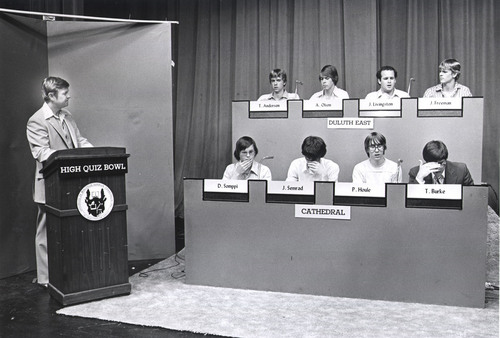
\includegraphics{qb/quizbowl}

	\end{columns}

\end{frame}
\begin{frame}[t]
	\frametitle{Sample Question}

        The Swiss-Italian architect Pietro Antonio Solari
        \only<2->{built several fortified towers in this city, which
          often vied for power with its northern rival Tver. A ruler
          of this city prevailed in the} \only<3->{Great Stand on the
          Ugra River. A prince from this city was nicknamed for
          winning a battle on the} \only<4->{Don river. Partly because
          a ruler of this city married} \only<5->{Sophia Palaiologina,
          the niece of the last Byzantine Emperor, this city styled
          itself the} \only<6->{``Third Rome'' after the fall of
          Constantinople. Another prince of this city stopped paying
          tribute to the} \only<7->{Mongols in 1476, ending the
          ``Tatar yoke.''} \only<8->{The Grand Duchy headquartered in
          this city came to an end in 1547 with the ascension of}
        \only<9->{ Ivan IV, who made it his capital. For 10 points,
          name this city where Ivan III renovated the
          Kremlin,} \only<10->{the capital of Russia.}\\
        \vspace{.5cm} \only<11->{ {\bf Moscow} (Moskva / Muscovy)}

\end{frame}


\begin{frame}
	\frametitle{Question Structure Enables Compeition}

	\begin{columns}
		\column{.5\linewidth}

		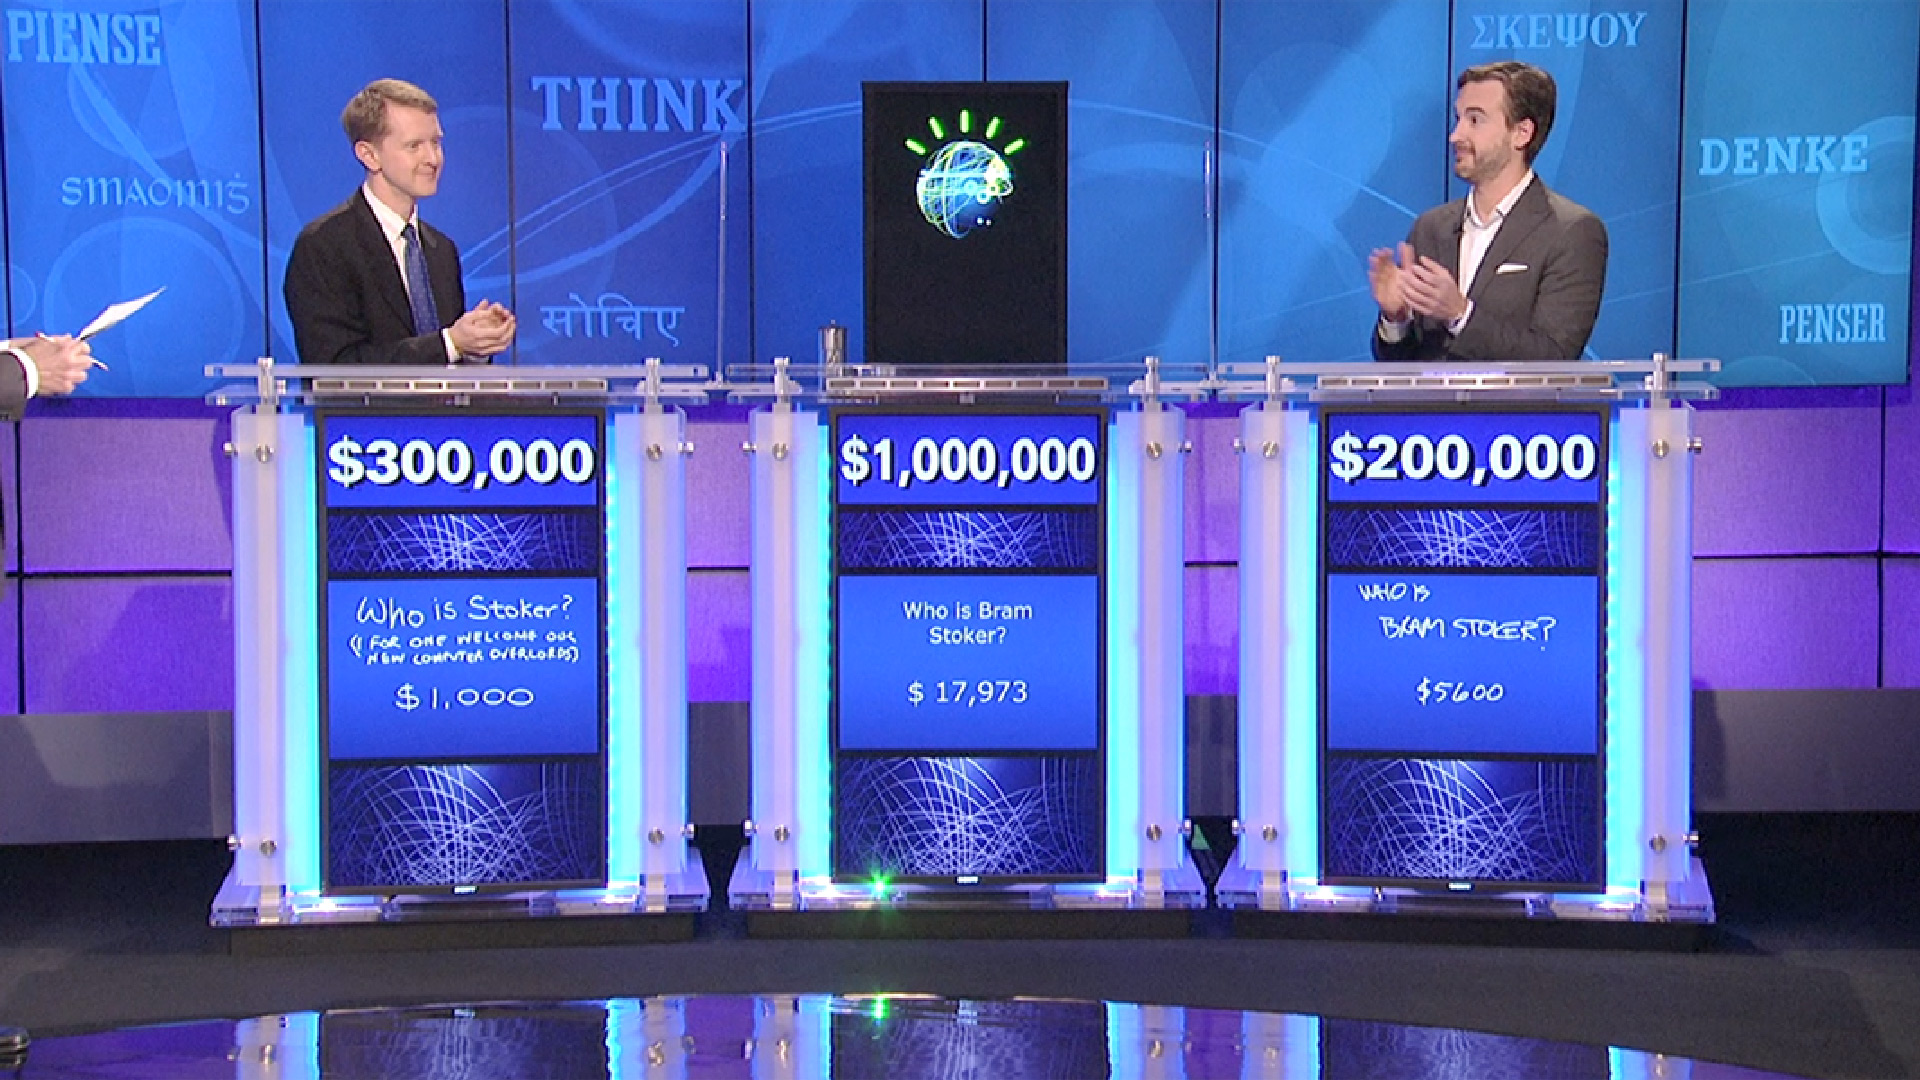
\includegraphics[width=1.0\linewidth]{qb/jeopardy}


		\column{.5\linewidth}
		\begin{itemize}
                        \item Watson must decide to answer {\bf once}, after
                          complete question
                        \item Quiz Bowl: decide after each word
                        \item Obscure clues at start, easy at end
                        \item ``Gold standard'' in trivia community: high school to college
		\end{itemize}

	\end{columns}

      \end{frame}

%       \begin{frame}{A Trivia Tournament is a Leaderboard!}
%         \begin{columns}
%           \column{.5\linewidth}
%           \gfxq{trivia_tournament_leaderboard}{.8}
%           \column{.5\linewidth}

%           \begin{itemize}
% \item Commission questions and answers
% \item Decide on rules and scoring
% \item Advertise, get participants
% \item Participants answer questions
% \item Induce a ranking over the participants
% \item Declare a winner
%           \end{itemize}
%         \end{columns}
%       \end{frame}

\begin{frame}{A Case for Quizbowl}

  \begin{itemize}
    \item Pyramidality ensures proportion of discriminative questions is near 1.0
    \item Editing process minimizes ambiguities and errors
    \item Clever, inventive writers
    \item Fun for participants and viewers
  \end{itemize}
\end{frame}


\begin{frame}{Can we improve QA systems?}

\begin{columns}
  \column{.6\linewidth}
     \gfxq{trick/pyramid}{.9}
     \column{.4\linewidth}
     \begin{itemize}
       \item Questions should be pyramidal
       \item But for whom?
         \begin{itemize}
           \item Quotes
           \item Reusing clues
         \end{itemize}
     \end{itemize}
\end{columns}
\end{frame}

\fsi{qb/jennings_handshake}{}


\begin{frame}{Trick me if you can\dots}

  \begin{itemize}
  \item Trivia writers create questions
  \item {\bf Current} explain why they answer (and when)
  \item Trivia writers make questions go from hard to easy (for both
    humans and computers)
    \pause
    \item \only<2>{PROFIT!} \only<3>{Better questions!}
  \end{itemize}

\end{frame}

% \begin{frame}{What do we mean by ``adversarial''?}

%   \gfxq{trick/flow_chart_horizontal_label}{1.0}

%   \begin{itemize}
%     \item Both neural and IR systems
%       \pause
%     \item Reason we need to have good explanations of QA
%   \end{itemize}

% \end{frame}

\fsi{qb/trick/brahms_0}{\href{http://write.qanta.org}{http://write.qanta.org}}
\fsi{qb/trick/brahms_1}{}
\fsi{qb/trick/brahms_2}{}
\fsi{qb/trick/brahms_3}{}
\fsi{qb/trick/brahms_4}{}
\fsi{qb/trick/brahms_5}{}


\fsi{qb/trick/round_one}{Just as easy for humans, harder for computers.}



\begin{frame}{Competition}

  \gfxq{trick/pace}{.8}

\begin{itemize}
  \item December 15: Seven top human teams, fourteen computer teams
  \item Top four teams from each ``division'' faced off against each
    other
    \pause
  \item All computer teams lost to human teams
    \pause
  \item But two games were really close; strongest system was based on BERT
  \item YouTube videos: \href{https://go.umd.edu/2018hcqa}{https://go.umd.edu/2018hcqa}
\end{itemize}

\end{frame}



\begin{frame}{Impossible Until the End}
\alert<3>{Ritchie Watson commended this play's historical accuracy for
  getting the price for a dozen eggs right---ten cents---to defend
  against Elizabeth Hardwick’s contention that it was a sentimental
  history.} \alert<4>{At the end of this play, a man wonders why a wheelchair is
at the top of a staircase, and} \alert<5>{Alexandra announces that she is leaving
her mother. Leo is pressured into stealing a set of valuable railroad
bonds in this drama. In this play, which takes its title from the Song
of Solomon,} Regina Hubbard schemes  \tdiamond{PineGreen}
\tcircle{PineGreen} to obtain a majority share in a cotton mill. For 10
points,  \tsquare{PineGreen}  \ttriangle{PineGreen} name this play by
Lillian Hellman. \\

\pause

\textbf{Answer}: The\ Little\ Foxes\\

\only<3>{Academic literature}
\only<4>{Vague plot summary}
\only<5>{Avoid last names}

\end{frame}

% Tricky and hard: F3 Question 25

\begin{frame}{Tricky and impossible for current systems}
In Our Town, a character  \ttriangle{BrickRed} with this given name explains Grover’s Corners’ place in the universe. In The Crucible, a character  \tcircle{BrickRed} with this first name contends that the girls’ actions are part of their “silly seasons” and is the wife of Francis Nurse. A novel with this name, which conducts hidden messages to Rommel in The English Patient, is titled for a character who is killed in a boating accident at Manderley. For 10 points, give this name of a Daphne du Maurier  \tdiamond{Goldenrod}  \tsquare{PineGreen} gothic novel which is also the first name of Miss Sharp, the protagonist of William Thackeray's Vanity Fair. \tcircle{gray}  \ttriangle{gray}


\ttriangle{BrickRed} Thornton Wilder
\tcircle{BrickRed} Richard
\tcircle{gray} Richard
\ttriangle{gray} Thornton Wilder \\
\textbf{Answer}: Rebecca\\
\end{frame}


\begin{frame}{Close, but \dots}
An army that took its name from this geographical feature had a
British doctor, James Paroissien, as its Surgeon General, and recent
scholarship by Peter Blanchard revealed its use of slaves. That army
crossed this geographical feature according  \ttriangle{BrickRed} to
Thomas Maitland’s  \tcircle{BrickRed} plans at Uspallata and Los
Patos. Spanish forces under Rafael Maroto were defeated in the
foothills of these mountains by an army led by José de San Martín and
Bernardo O'Higgins.  \tsquare{BrickRed} For 10 points, name this mountain
range of South America that played a role  \ttriangle{Goldenrod} in the
independence of Chile. \tdiamond{gray}  \tcircle{gray}  \tsquare{gray}

\ttriangle{BrickRed} Angel Falls
\tcircle{BrickRed} Mountain
\tsquare{BrickRed} Battle of Chacabuco
\tdiamond{gray} Battle of Chacabuco
\tcircle{gray} Mountain
\tsquare{gray} Battle of Chacabuco \\
\pause
\textbf{Answer}: Andes\\

\end{frame}


\begin{frame}{Linguistics FTW}

  The main character of a story by \alert<2>{this author opens Crime and Punishment} to a
random page, but finds it to be a copy of The Brother Karamazov, and equates
himself with Monsieur Bovary. This author wrote a story in which the priest
Naigu undergoes a boiling treatment to decrease the size of his nose. This
author of "Cogwheels" wrote about two people who steal to survive near the
southern gate of Kyoto in a story that features inconsistent accounts from a
woodcutter, a priest, a widow, and the ghost of a samurai. For 10 points, name
this author of "Rashomon" and namesake of a Japanese literary prize. \\
\only<3->{\textbf{Answer}: Ryunosuke Akutagawa}
\end{frame}



\begin{frame}[plain]
\gfxq{seattle_crowd}{.5}
\gfxq{chicago_crowd}{.5}
\end{frame}

\fsi{qb/boring_dot_products}{}

\fsi{simtrans/centaur-chess}{Centaur Chess}

\begin{frame}{Opportunities for Education}

  \begin{itemize}
  \item Undergrads can build their own systems
  \item Contributions outside of computer science
  \item How smart humans are, how dumb computers are
  \item A fun spectacle!
  \end{itemize}

\end{frame}

\begin{frame}{So much left to do!}

  \begin{itemize}
  \item Annual evaluations
  \item Better representation: 90\% of SQuAD questions about men
  \item Multilingual: Need to actually represent culture and langauge
  \item Combine with speech recognition
  \end{itemize}
  
\end{frame}

\begin{frame}{Imitation Game}

  I believe that in about fifty years’ time it will be possible to programme computers, with a storage capacity of about 109, to make them play the imitation game so well that an average interrogator will not have more than 70 percent chance of making the right identification after five minutes of questioning. … I believe that at the end of the century the use of words and general educated opinion will have altered so much that one will be able to speak of machines thinking without expecting to be contradicted.

\end{frame}

\fsi{qb/turing}{Turing Test: Definition of AI (Image from Wall Street
  International)}

\begin{frame}{Why not a game show?}

  \begin{itemize}
  \item Bring community together
  \item Force people to look at the data
  \item Fair human comparisons
  \item Slowly increase the difficulty
  \end{itemize}

\end{frame}



\frame{
  \frametitle{But wait, there's more!}

  \vspace{-.5cm}

\begin{columns}



  \column{.5\linewidth}

   \begin{block}{Computational Social Science}
     \centering
     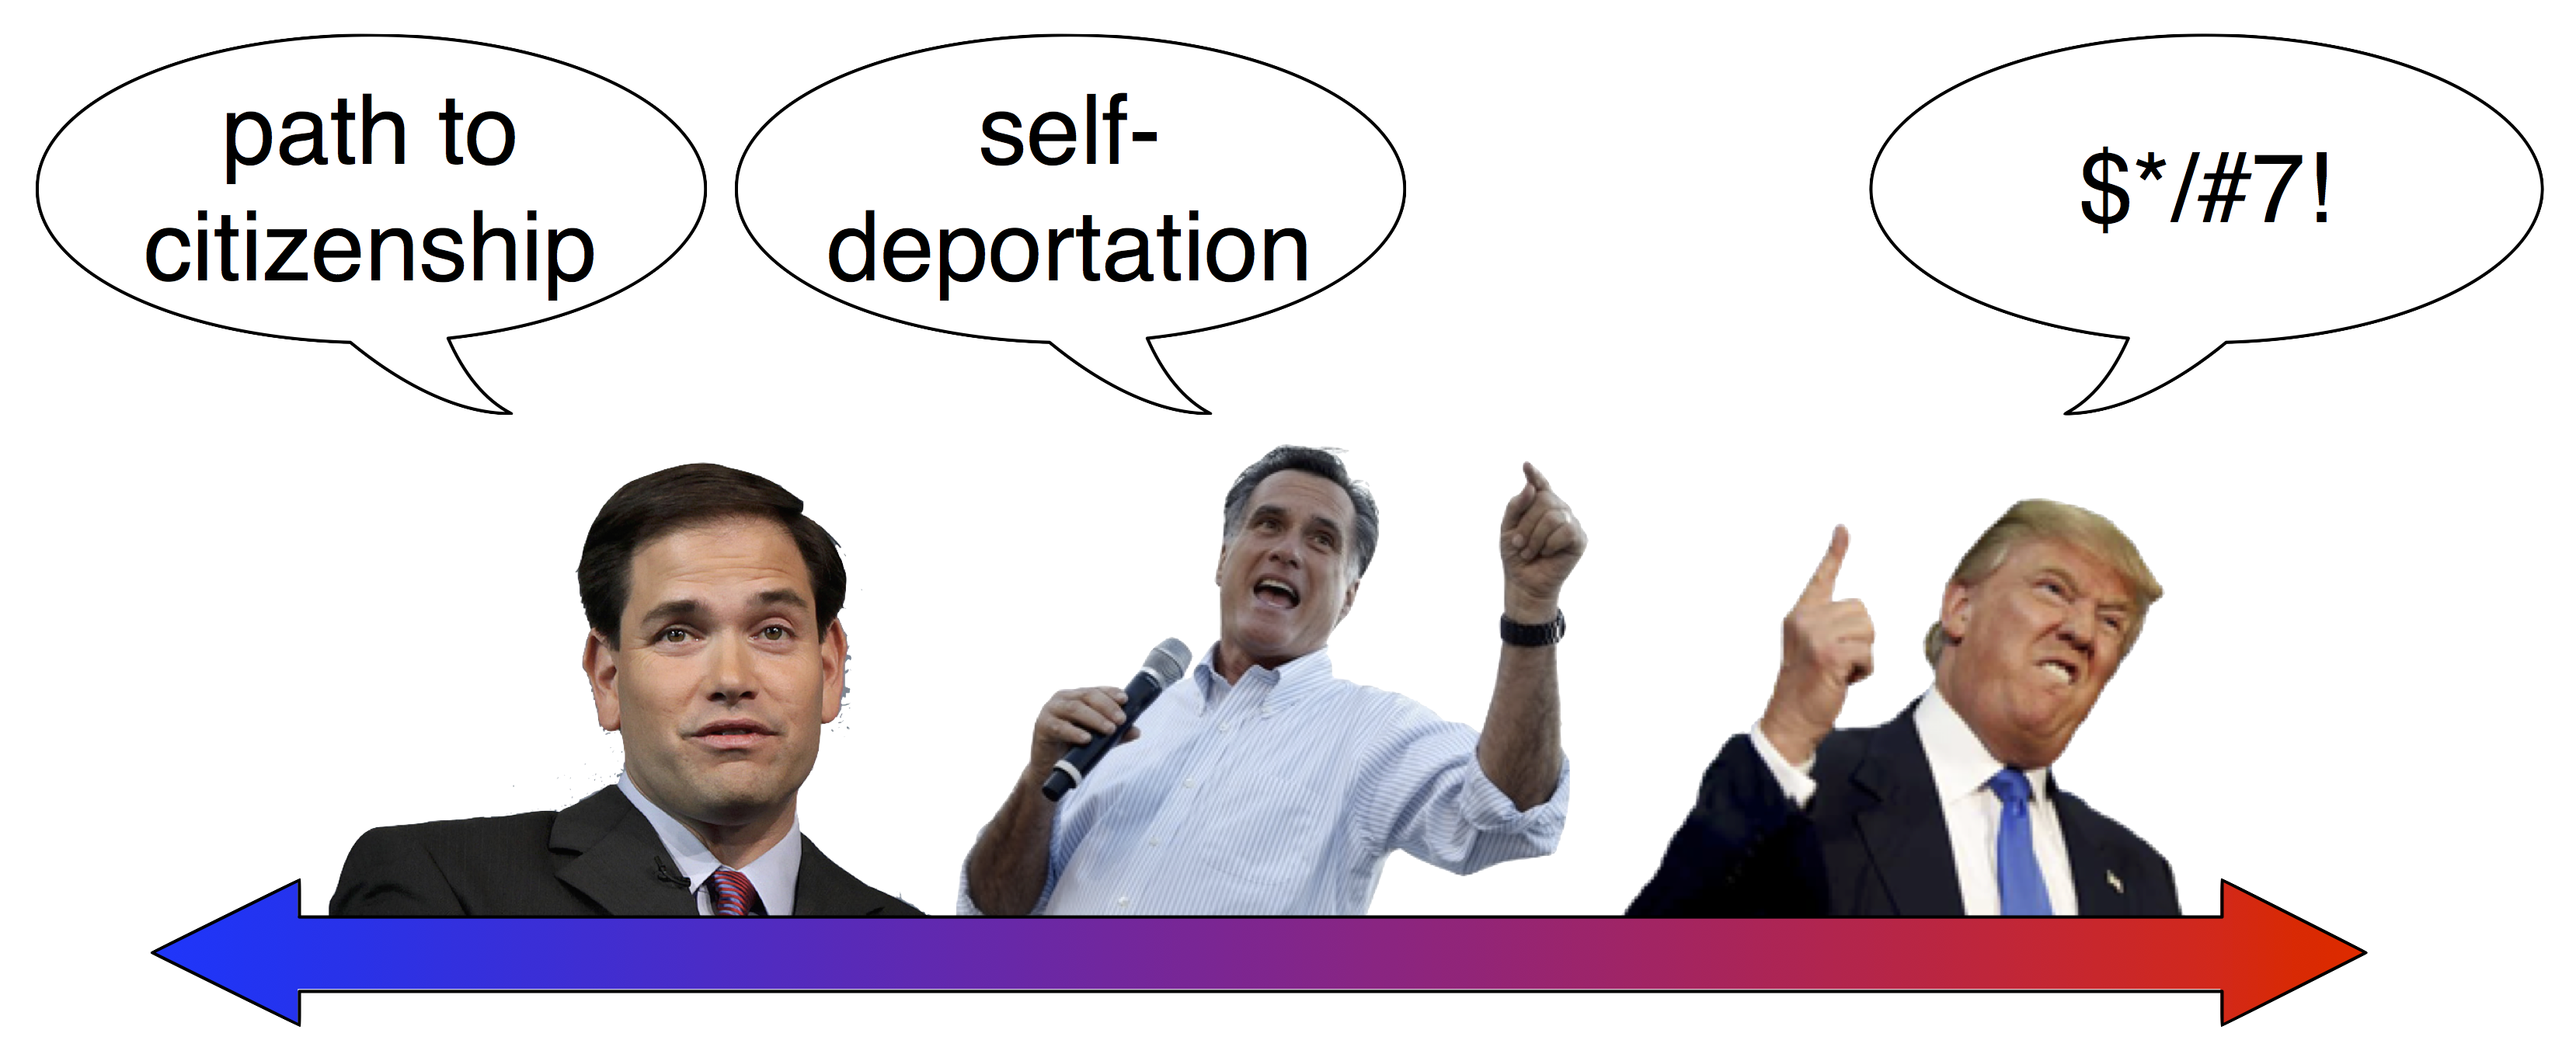
\includegraphics[width=0.9\linewidth]{teaparty/figures/framing} \\
     \cite{nguyen-13b,nguyen-15}
   \end{block}


    \begin{block}{Interactive Machine Learning}
     \centering
        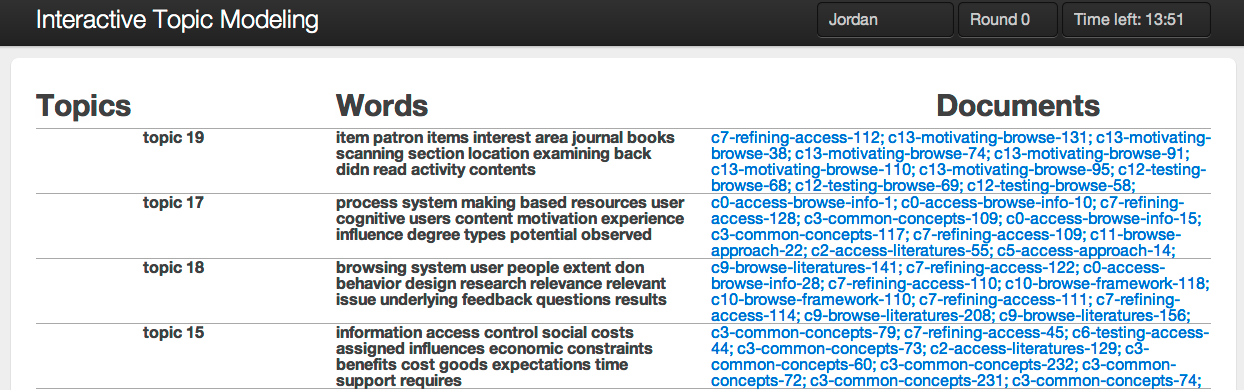
\includegraphics[width=0.4\linewidth]{interactive_topic_models/new_interface} \\
       \cite{Smith-17,Poursabzi-16}
    \end{block}


  \column{.5\linewidth}


    \begin{block}{Multilingual Topic Models}
      \begin{center}
        \begin{large}
          $p_{\mbox{topic}}(e | f)$ \\
         \end{large}
      \cite{eidelman-12,hu-14}
       \end{center}
    \vspace{-.3cm}
    \end{block}


    \begin{block}{Sentiment / Internal State}
    \centering
        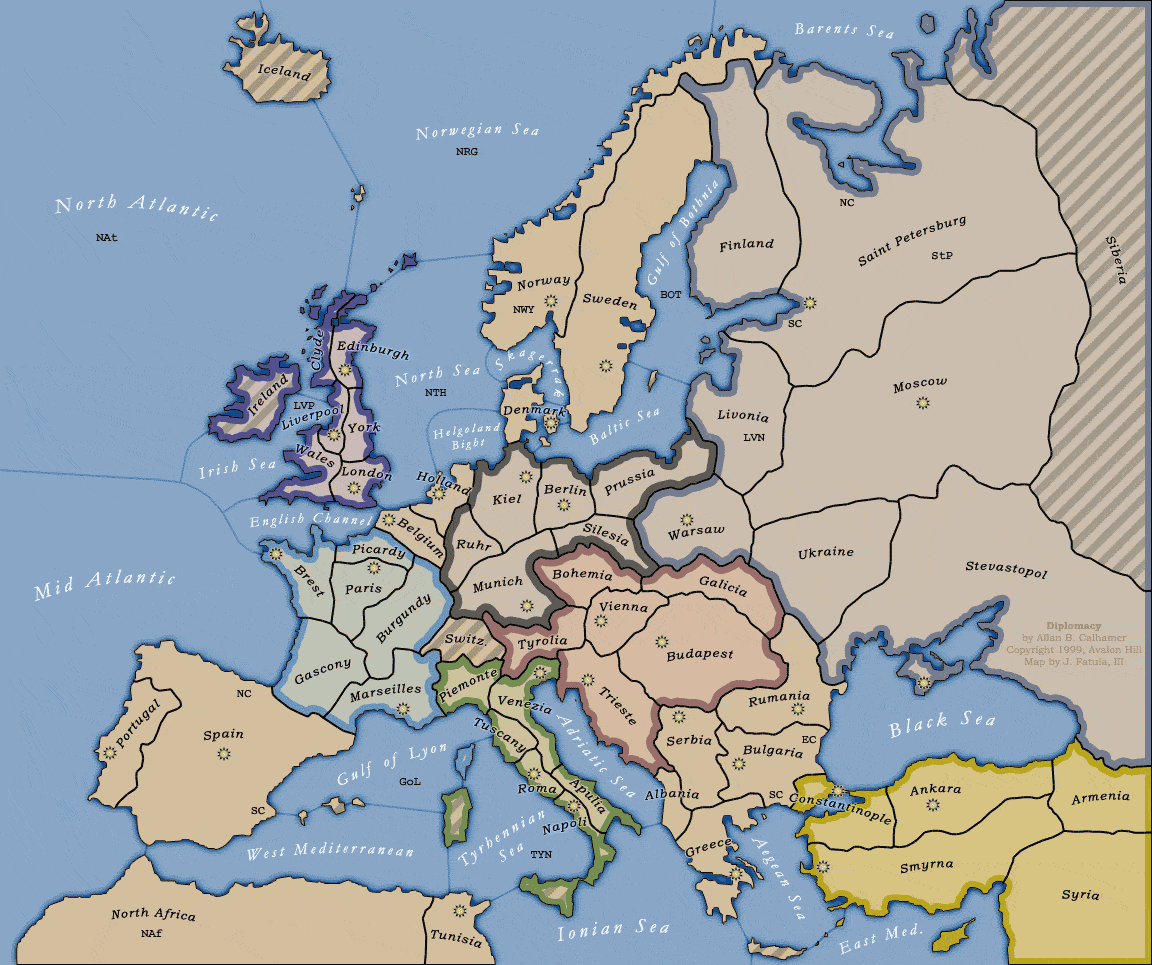
\includegraphics[width=0.4\linewidth]{general_figures/diplomacy} \\
        \cite{niculae-15,sayeed-12,boyd-graber-10}
    \end{block}




\end{columns}

}

\begin{frame}{Sabotaged by IR}

  \rowcolors{2}{gray!25}{white}
  \begin{small}
  \begin{tabular}{p{7cm}p{3cm}}
    \toprule
    Question & Page \\
    \hline
 when did the states secede during the civil war &  Border states (American Civil War) \\
 who wears number 2 for the dallas cowboys &  Jeff Heath (American football) \\
 how many countries participated for the first time in the 2014 olympic winter games in sochi & 2014 Winter Paralympics \\
 game of thrones season 7 number of episoded &  List of Teen Wolf episodes \\
 \bottomrule
  \end{tabular}
  \end{small}

\end{frame}

\begin{frame}{Good for Search, Bad for QA}

  Title of page is answer, annotators didn't find span:
  \rowcolors{2}{gray!25}{white}
  \begin{tabular}{p{7cm}p{3cm}}
    \toprule
    Question & Page \\
    \hline
  who plays the goblin king in the hobbit &  Barry Humphries  \\
  who does the voice of fart in rick and morty & Jemaine Clement   \\
 \bottomrule
  \end{tabular}
\end{frame}

\begin{frame}{Questions Depends on Who / When}
  \rowcolors{2}{gray!25}{white}
  \begin{tabular}{p{8cm}p{2cm}}
    \toprule
    Question & Gold Answer \\
    \hline
    can i buy wine in kentucky on sunday & --- \\
    where am i on the steelers waiting list & --- \\
    when is the real housewives on & --- \\
    who has majority in the house and senate & --- \\
    \bottomrule
  \end{tabular}  

  \pause

  \begin{block}{Answerable Questions\dots}
  But depend on which county of Kentucky you're in,
  when you paid for your season pass, and the local network
  syndicating Real Housewives.
  \end{block}
  
\end{frame}


\begin{frame}{References}
\bibliographystyle{style/acl}
\tiny
\bibliography{bib/journal-full,bib/jbg}
\end{frame}



\end{document}